\documentclass[12pt]{article}

\usepackage{amsmath,amsthm,amsfonts,amssymb,amsxtra}
\usepackage{pgf,tikz}
\usetikzlibrary{arrows}

\renewcommand{\theenumi}{(\alph{enumi})} 
\renewcommand{\labelenumi}{\theenumi}

\pagestyle{empty}
\setlength{\textwidth}{7in}
\setlength{\oddsidemargin}{-0.5in}
\setlength{\topmargin}{-1.0in}
\setlength{\textheight}{9.5in}

\theoremstyle{definition}
\newtheorem{problem}{Problem}

% Points, objects
\def\v{\boldsymbol{v}}
\def\w{\boldsymbol{w}}
\def\x{\boldsymbol{x}}
\def\y{\boldsymbol{y}}
\def\z{\boldsymbol{z}}
\def\e{\boldsymbol{e}}
\def\xstar{\boldsymbol{x}^{\star}}
\def\field#1{\mathbb{#1}}
\def\ball#1{\field{B}^{#1}} 
\def\sphere#1{\field{S}^{#1}}
\def\open#1{\overset{\mathrm{o}}{#1}}

% Functions
\def\supp{\operatorname{supp}}
\def\sign{\operatorname{sign}}
\def\ceil#1{\lceil{#1}\rceil} 
\def\floor#1{\lfloor{#1}\rfloor}
\def\epi{\operatorname{epi}} 
\DeclareMathOperator*{\argmin}{arg\,min}

% Functionals, norms
\def\abs#1{\lvert #1 \rvert} 
\def\norm#1{\lVert #1 \rVert}
\def\dist{\operatorname{d}}
\def\gradient#1{\mathop{\nabla\! {#1}}}
\def\Hess#1{\mathop{\mathrm{Hess}{#1}}}

\begin{document}

\noindent{\large\bf MATH 524}\hfill{\large\bf Exam \#1.}\hfill{\large\bf
  Fall 2017}\hfill{\large\bf Page 1/4}\hrule

\bigskip
\begin{center}
  \begin{tabular}{|ll|}
    \hline & \cr
    {\bf Name: } & \makebox[12cm]{\hrulefill}\cr & \cr
    {\bf VIP ID:} & \makebox[12cm]{\hrulefill}\cr & \cr
    \hline
  \end{tabular}
\end{center}
\begin{itemize}
\item Write your name and VIP ID in the space provided above.
\item The test has four (4) pages, including this one. 
\item You must show sufficient work to justify all answers unless otherwise stated in the problem.  Correct answers with inconsistent work may not be given credit.
\item Credit for each problem is given in parentheses at the right of the problem number.
\end{itemize}
\hrule

\begin{center}
  \begin{tabular}{|c|c|c|}
    \hline
    &&\cr
    {\large\bf Page} & {\large\bf Max.~points} & {\large\bf Your points} \cr
    &&\cr
    \hline
    &&\cr
    {\Large 2} & \Large 50 & \cr
    &&\cr
    \hline
    &&\cr
    {\Large 3} & \Large 30 & \cr
    &&\cr
    \hline
    &&\cr
    {\Large 4} & \Large 20 & \cr
    &&\cr
  \hline\hline
    &&\cr
    {\large\bf Total} & \Large 100 & \cr
    &&\cr
    \hline
  \end{tabular}
\end{center}
\newpage

%%%%%%%%%%%%%%%%%%%%%%%%%%%%%%%%%%%%% Page 2
\noindent{\large\bf MATH 524}\hfill{\large\bf Exam \#1.}\hfill{\large\bf
  Fall 2017}\hfill{\large\bf Page 2/4}\hrule

\bigskip
\begin{problem}[50 pts---10 pts each part]
Consider the 2nd-degree polynomial 
\begin{equation*}
p_2(x,y) = 4x^2 + 25y^2 - 20xy.
\end{equation*}
\begin{enumerate}
  \item The polynomial $p_2$ is a quadratic form.  Find a symmetric matrix $\boldsymbol{A}$ so that 
  \begin{equation*}
  p_2(x,y) = \mathcal{Q}_{\boldsymbol{A}}(x,y).
  \end{equation*}
  \begin{proof}[Solution] Directly from the coefficients of $p_2$ we obtain $ \boldsymbol{A} = \begin{bmatrix} 4 & -10 \\ -10 & 25 \end{bmatrix}$.\end{proof}
  \item Classify the symmetric matrix $\boldsymbol{A}$.
  \begin{proof}[Solution]
  We can do this by using the \emph{Principal Minor Criteria}, or the \emph{Eigenvalue Criteria}.
  For instance, with the former: $\Delta_1 = 4 > 0$, $\Delta_2 = 0$.
  With the latter:
  \begin{equation*}
  \det \begin{bmatrix} 4-\lambda & -10 \\ -10 & 25-\lambda \end{bmatrix} = (4-\lambda)(25-\lambda) - 100 = \lambda^2-29\lambda = \lambda(\lambda-29)
  \end{equation*}
  In each case we obtain the same answer: this matrix is positive semi-definite. \end{proof}
  \item Sketch the level line $p_2(x,y) = 0$.  
  \begin{proof} Note that $4x^2+25y^2=20xy = (2x-5y)^2$.  The level line is thus $2x-5y=0$, or $y=\tfrac{2}{5}x$.\end{proof}
  \begin{center}
  \begin{tikzpicture}[scale=0.75]
  \draw [ultra thick] (-3,-3) rectangle (3,3);
  \draw [ultra thick] (-3,0) -- (3,0);
  \draw [red] (-3,-1.2) -- (3,1.2);
  \draw [fill=red] (2.5,1) circle (3pt) node[above, red] {$(5,2)$};
  \draw [ultra thick] (0,-3) -- (0,3);
  \draw [thin, step=0.5, gray] (-3,-3) grid (3,3);
  \end{tikzpicture}
  \end{center}
  \item Is $p_2$ a coercive function?  Why?
  \begin{proof}[Solution]  Notice $p_2\big(x,\tfrac{2}{5}x\big)=0$ for all $x \in \field{R}$.  This polynomial is not coercive. \end{proof}
  \item Find all critical points of $p_2$, and classify them.
  \begin{proof}[Solution]
  The gradient of $p_2$ is $\gradient{p_2}(x,y) = \big[ 8x -20y, 50y - 20 x \big]$.  Solving $\gradient{p_2}(x,y) = \boldsymbol{0}$ gives all the points on the line $y = \tfrac{2}{5}x$.  Notice how, at all points $(x,y)$ (not only on that line), the Hessian is positive semi-definite:
  \begin{equation*}
  \Hess{(p_2)} (x,y ) = \begin{bmatrix} 8 & -20 \\ -20 & 50 \end{bmatrix} = 2 \boldsymbol{A}.
  \end{equation*}
  Those points are therefore all global minima of the function $p_2$.
  \end{proof}
\end{enumerate}
\end{problem}

\newpage


%%%%%%%%%%%%%%%%%%%%%%%%%%%%%%%%%%%%% Page 3
\noindent{\large\bf MATH 524}\hfill{\large\bf Exam \#1.}\hfill{\large\bf
  Fall 2017}\hfill{\large\bf Page 3/4}\hrule

\bigskip
\begin{problem}[30 pts---10 pts each part]
Consider the function
\begin{equation*}
f(x,y,z) = x^2+y^2+z^2 + \frac{1}{x^2+y^2+z^2}
\end{equation*}
\begin{enumerate}
  \item Is $f$ a convex function?  Why?
  \begin{proof}[Solution]
  Notice we may write $f(x,y,z) = (g\circ h) (x,y,z)$, where $h(x,y,z) = x^2+y^2+z^2$ for $(x,y,z) \in \field{R}^3$ and $g(t) = t+\tfrac{1}{t}$ for $t \in (0,\infty)$.  Both $h$ and $g$ are strictly convex functions. For instance, the Hessian of $h$ at any point $(x,y,z)$ is positive definite:
  \begin{equation*}
  \Hess{h}(x,y,z) = \begin{bmatrix} 2 & 0 & 0 \\ 0 & 2 & 0 \\ 0 & 0 & 2 \end{bmatrix}; \quad \lambda_1 = \lambda_2 = \lambda_3 = 2 >0
  \end{equation*}
  The second derivative of $g$ is always positive in $(0,\infty)$: $g'(t) = 1- t^{-2}$, $g''(t) = 2t^{-3}$.  
  \end{proof}
  \item What is the global minimum value of $f$?  Why?
  \vspace{1cm}
  \item Find all global minima of $f$.
\end{enumerate}
\end{problem}
\newpage

%%%%%%%%%%%%%%%%%%%%%%%%%%%%%%%%%%%%% Page 4
\noindent{\large\bf MATH 524}\hfill{\large\bf Exam \#1.}\hfill{\large\bf
  Fall 2017}\hfill{\large\bf Page 4/4}\hrule

\bigskip
\begin{problem}[20 pts]
Consider the function $f(x,y)= x^3+e^{3y}-3xe^y$.  Show that $f$ has exactly one critical point, and that this point is a local minimum but not a global minimum.
\begin{proof}[Solution]
It is easy to see that this function does not have a global minimum.  For instance, if $y=0$ we have $f(x,0)=x^3-3x+1$, a polynomial of degree 3: 
\begin{equation*}
\lim_{x\to -\infty} f(x,0)= -\infty.
\end{equation*}
The gradient of $f$ is $\gradient{f}(x,y) = \big[ 3x^2-3e^y, 3e^{3y}-3xe^y \big]$.  Solving $\gradient{f}(x,y) = \boldsymbol{0}$ gives the equations
\begin{equation*}
\begin{cases}  x^2-e^y=0, \\ e^{2y}-x=0, \end{cases}
\end{equation*}
which resolves in the only point $(1,0)$ (since it must be $x=e^{2y}$, and thus $e^{4y}-e^y=0$, which results in $e^y=1$, or $y=0$)  To see that this point is a strict local minimum, we check the Hessian at that location:
\begin{equation*}
\Hess{f}(1,0) = \begin{bmatrix} 2 & -1 \\ -1 & 2 \end{bmatrix}; \quad \Delta_1 = 2 > 0, \quad \Delta_2 = 3 > 0. \qedhere
\end{equation*}
\end{proof}
\end{problem}

\end{document}
